\addtotoc{Товчлол}
\thispagestyle{plain}

\vspace*{-6mm}
\begin{center}
\textbf{\large \titlename}\\[1mm]
\end{center}

\begin{flushright}
\departmentname\\
Оюутан: \studentID, \authorShort\\
Удирдагч багш: \supervisorname
\end{flushright}

\vspace{1mm}
\setcounter{table}{0}
\setcounter{figure}{0}
\renewcommand{\thetable}{\arabic{table}}
\renewcommand{\thefigure}{\arabic{figure}}
\setlength{\columnsep}{7mm}
\begin{multicols}{2}
\setlength{\parskip}{5pt}
\sloppy

\noindent\textbf{1. Удиртгал}

Энэхүү дипломын ажил нь оюутны суралцах үйл явц дахь мэдлэгийн хуваагдмал байдал, мэргэжлийн нэр томьёоны ойлголтын хүндрэл, бүтээлийн баримтжуулалтын сул талыг бууруулах зорилготой FutureHub нэртэй нэгдсэн дижитал платформын суурь шийдлийг боловсруулж, хэрэгжүүлсэн. Систем нь веб платформ болон мобайл аппликейшныг нэг өгөгдлийн цөм дээр уялдуулж, мэдлэг хуримтлуулах, давтах, хуваалцах, үнэлэгдэх урсгалыг нэг дор төвлөрүүлэхэд чиглэсэн.

Судалгааны зорилт нь: (1) SRS суурьтай флашкартын урсгалыг хэрэгжүүлэх, (2) OCR болон толь бичгийн интеграц бүхий мэдлэгийн нэгтгэл бий болгох, (3) нийтлэл, Q\&A, project log зэрэг хамтын контентын орчныг хөгжүүлэх, (4) хэрэглэгчийн оролцоог ранкинг ба портфолиогоор хэмжиж үнэлэх, (5) системийн шийдлийг туршилтын түвшинд баталгаажуулах.

\noindent\textbf{2. Онолын суурь}

Судалгааны онолын суурь нь Spaced Repetition System (SM-2), хамтын мэдлэгийн системийн хандлага (Q\&A, нийтлэл, moderation), OCR технологи (ML Kit, Tesseract.js), мөн contribution-based үнэлгээний загварт тулгуурласан. Эдгээр онол, технологийн хослол нь зөвхөн мэдээлэл хадгалах бус, мэдлэгийг тогтоох, хэрэглээ болгох, дараа нь нийгэмлэгт буцаан хуваалцах мөчлөгийг бүрдүүлэх үндэс болсон.

\begin{center}
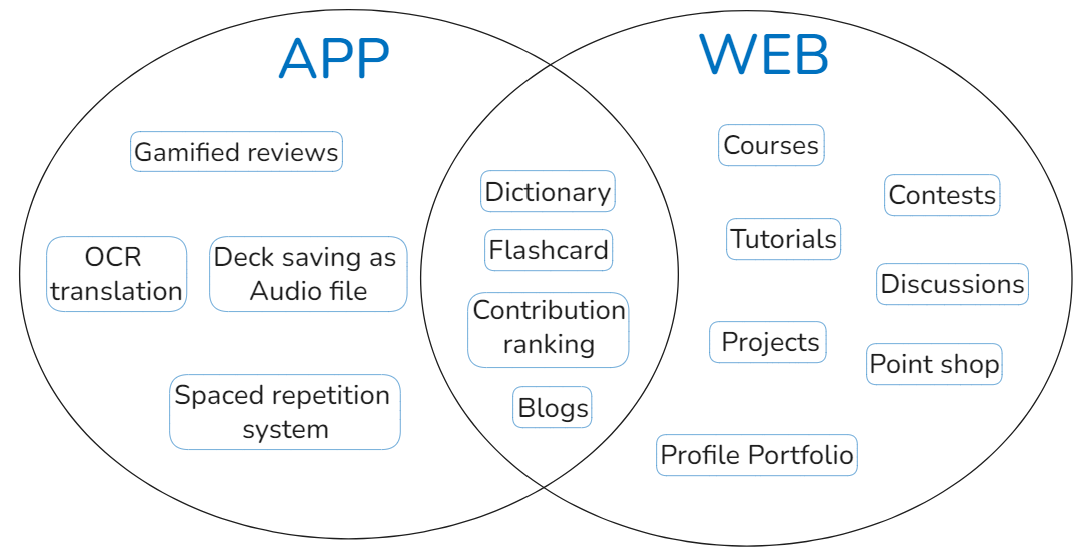
\includegraphics[width=0.95\linewidth]{pictures/functions-diagram.png}
\captionof{figure}{Веб ба мобайл функцийн огтлолцол}
\label{fig:brief-function-venn}
\end{center}

\noindent\textbf{3. Арга зүй}

Системийг Iterative SDLC загвараар хэрэгжүүлж, шаардлага тодорхойлох, модульчлан хөгжүүлэх, интеграцчлах, турших үе шатыг давтамжтайгаар сайжруулсан. Архитектурын түвшинд Next.js (веб), Flutter (мобайл), Supabase/PostgreSQL (backend, өгөгдлийн сан)-ийг нэгдсэн байдлаар ашигласан.

Арга зүйн хүрээнд core (флашкарт, толь бичиг, Q\&A, нийтлэл) болон extended (тэмцээн, сургалт, ранкинг, аналитик) шаардлагыг ялган загварчилж, хэрэглэгчийн үүргээр (оюутан, багш, админ) матрицчилсан. Туршилтыг unit, integration, UAT гэсэн гурван түвшинд зохион байгуулж, SRS интервал тооцоолол, OCR урсгал, RLS эрхийн хязгаарлалт, модуль хоорондын өгөгдлийн уялдааг шалгасан.

\begin{center}
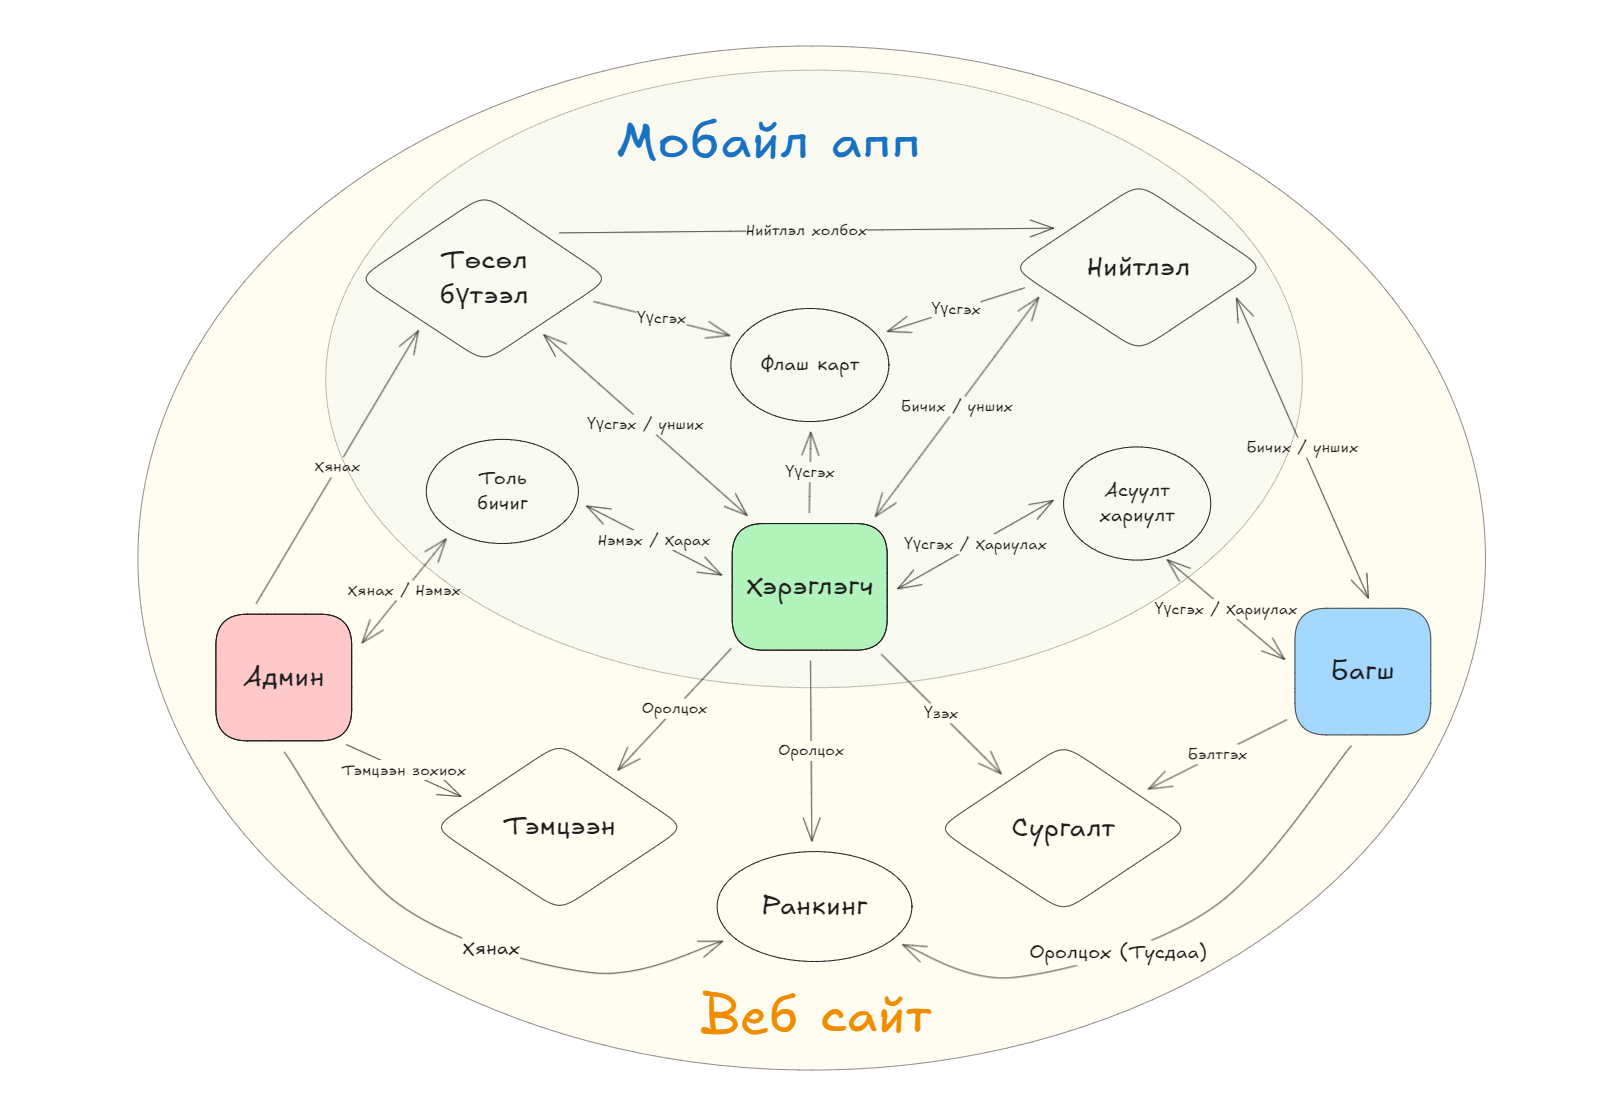
\includegraphics[width=0.95\linewidth]{pictures/futurehub-context.png}
\captionof{figure}{FutureHub системийн context diagram}
\label{fig:brief-context-diagram}
\end{center}

\noindent\textbf{4. Үр дүн ба дүгнэлт}

Хэрэгжилтийн үр дүнд FutureHub-ийн үндсэн долоон модуль (Flashcard, Dictionary, Article/Blog, Discussion, Project Log, Contest/Course, Ranking) бодитой ажиллах түвшинд нэгтгэгдсэн. Веб талд контент үүсгэх, баталгаажуулах, хэлэлцүүлэх, удирдах боломж бүрдсэн бол мобайл талд SRS давталт, OCR-оор карт үүсгэх урсгал хэрэгжсэн.

Туршилтын дүнгээр толь бичгээс карт үүсгэх, нийтлэл нийтлэх, project log-профайл уялдаа, contribution ranking шинэчлэлт, SRS интервалын тооцоолол, RLS хамгаалалтын үндсэн кейсүүд амжилттай баталгаажсан. OCR урсгал нь сайн гэрэлтүүлэгтэй зураг дээр өндөр нарийвчлалтай ажилласан боловч гар бичмэл болон чанар муутай зураг дээр хэрэглэгчийн засвар шаардлагатай хэвээр байгааг тогтоосон. API-ийн дундаж хариу өгөх хугацаа зорилтот 500 мс босгоос доогуур гүйцэтгэлтэй байсан.

Ерөнхийд нь, FutureHub нь суралцах, мэдлэг хуваалцах, хувь нэмрийг үнэлэх процессыг нэгтгэсэн боловсролын технологийн суурь экосистем болох боломжтойг харуулсан.

\begin{center}
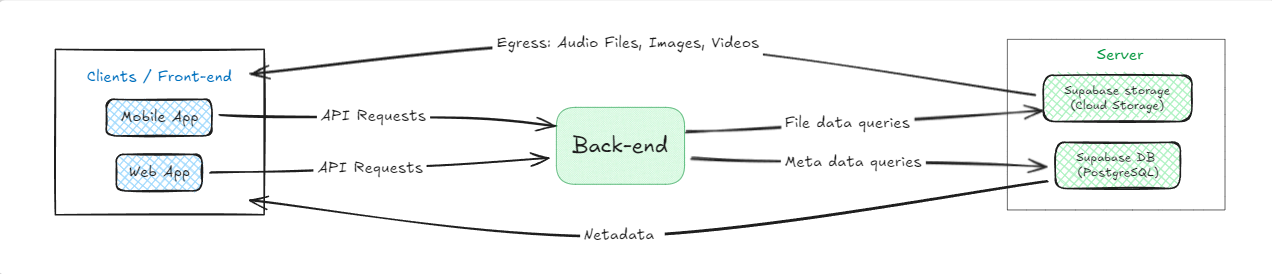
\includegraphics[width=0.95\linewidth]{pictures/system-architecture.png}
\captionof{figure}{FutureHub системийн архитектурын зураглал}
\label{fig:brief-system-architecture}
\end{center}

\begin{center}
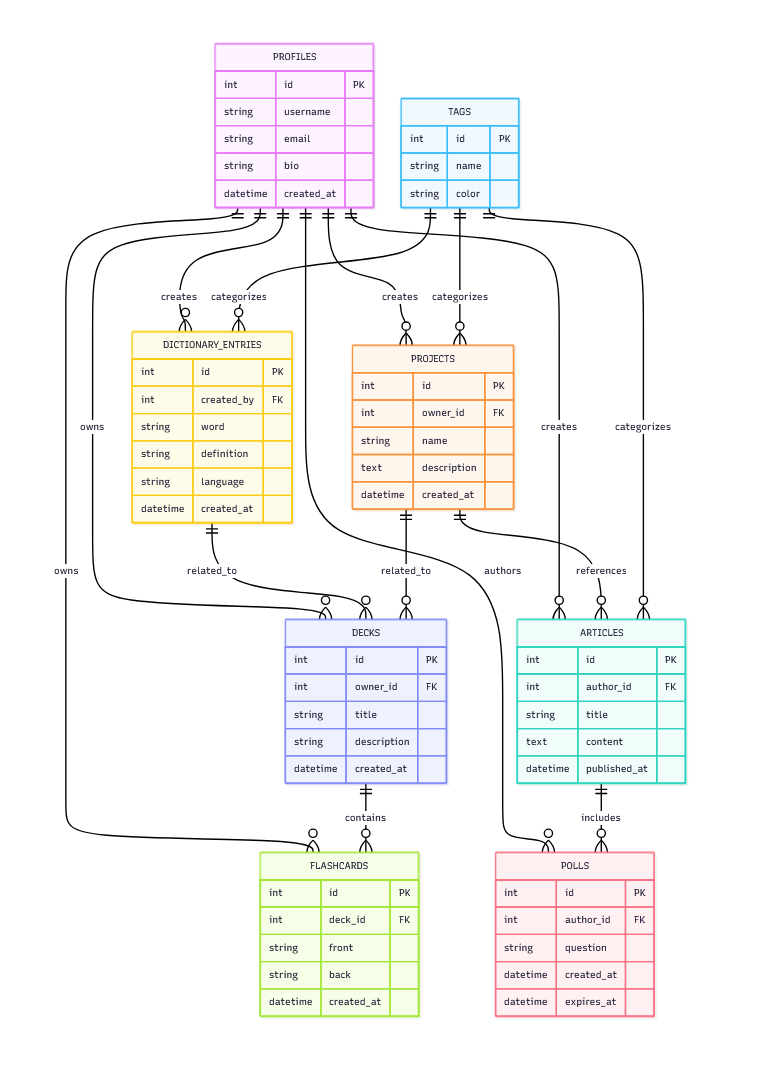
\includegraphics[width=0.95\linewidth]{pictures/general-erdiagram.png}
\captionof{figure}{FutureHub системийн ER диаграм}
\label{fig:brief-er-diagram}
\end{center}

\noindent\textbf{5. Ном зүй}

\small
Товчлолын гол эх сурвалжууд:
\begin{enumerate}
    \item Wozniak, P. A. (1990). Optimization of Learning (SM-2 algorithm).
    \item Baeza-Yates, R., \& Ribeiro-Neto, B. (2011). Modern Information Retrieval.
    \item PostgreSQL Global Development Group. Full-text Search Documentation.
    \item Google. ML Kit Text Recognition Documentation.
    \item Supabase Documentation (Auth, RLS, PostgreSQL integration).
    \item Next.js, Flutter official technical documentation.
\end{enumerate}
\normalsize

\end{multicols}
